\chapter{Gestión del proyecto}

El actual capítulo describe la gestión del proyecto, incluyendo ciclo de vida, planificación o un detalle del presupuesto.

\section{Ciclo de vida}

La práctica totalidad de los proyectos que se pueden imaginar son divisibles en etapas. La división proporciona un orden al desarrollo y evita descordinaciones, resultando vital al hablar de trabajo en equipo.

El presente proyecto no es menos y ha sido realizado acorde a una organización establecida. En primera instancia, se han desarrollado bloques de trabajo generados a partir del agrupamiento de tareas con un fin similar. Dentro de las tareas muy posiblemente se podrían definir subtareas anidadas de tal forma que es posible atomizar el trabajo.

La organización base de estos bloques de tareas queda recogida en el Diagrama de Pert de la figura \ref{fig:pert}\footnote{Los tiempos de inicio, duración y final indicados en los nodos están expresados en semanas}. Un diagrama de este estilo debe interpretarse de tal manera que una etapa apuntada por una o varias flechas no puede pasar a ser ejecutada mientras las etapas que le apuntan aún no hayan sido finalizadas, es decir, la flechas generan relaciones de dependencia entre los bloques de tareas presentados.

El Diagrama de Pert se traza de acuerdo a un ciclo de vida ideal que, a la hora de la verdad, no debe ser rígido. Esa es la razón por la que es posible comenzar a trabajar ciertos bloques de tareas sin respetar a raja tabla la dependencia de las flechas ya que pueden existir subtareas del bloque que no respondan a esta dependencia, excepcionalmente.

A continuación, se exponen los distintos grupos de tareas definidos en el diagrama de Pert:

\begin{itemize}
\item \textbf{Reacondicionamiento RHA}

La primera tarea es valorar el estado de la base del proyecto. Hay que detectar defectos y proponer y ejecutar soluciones a esos defectos con el fin de obtener un prototipo lo más funcional posible como base del proyecto.

\item \textbf{Comunicación Inicial XBees}

Comenzar en el mundo XBee requiere de pruebas y tiempo. Tanto es así que es consecuente definir una etapa cuyo único objetivo sea conocer los parámetros configurables de los módulos y establecer conexiones básicas con distintos firmwares.

\item \textbf{Comunicación definitiva XBees}

Posteriormente, se pueden definir los detalles de la configuración de los módulos orientados a la aplicación que se tiene en mente. Tras este proceso, deberían generarse los perfiles de comunicación.

\item \textbf{Integración XBee - RHA}

En esta etapa se deben explorar las formas de usar XBee en Arduino. Afortunadamente, es un tema cuya documentación y comunidad abunda en internet.

\item \textbf{Comunicación Arduino - RPi}

Este módulo incluye una primera comunicación remota entre el ordenador y el microcontrolador usados en el proyecto vía radiofracuencia. Se orienta al desarrollo inicial de software que trabaje en la comunicación.

\item \textbf{Comunicación Node-RED - XBee}

Se deben considerar todas las opciones disponibles para conectar módulos XBee a la Raspberry Pi y hacerlos interactuar con Node-RED

\item \textbf{Desarrollo Node-RED}

En este bloque se incluyen todas las tareas relacionadas con el desarrollo de los flujos de Node-RED para el control del brazo. Esto incluye el diseño de la interfaz gráfica.

\item \textbf{Interfaz MQTT}

Se añade la funcionalidad de controlar el brazo desde cualquier dispositivo con una conexión a la red MQTT, codificando el mensaje.

\item \textbf{Pruebas finales}

Se realiza el montaje final del prototipo y se comprueba que todas sus etapas reaccionan de manera adecuada.

\item \textbf{Desarrollo de la memoria}

A lo largo de gran parte del proyecto, se va desarrollando la presente memoria y documentación relacionada así como la recogida de datos experimentales para la demostración de resultados.

\item \textbf{Preparación Defensa TFG}

La última fase del proyecto corresponde a la preparación de la defensa del Trabajo Final de Grado, incluyendo el desarrollo de material visual de apoyo.

\end{itemize}

\begin{landscape}
   	\begin{figure}[H]
   		\centering
   		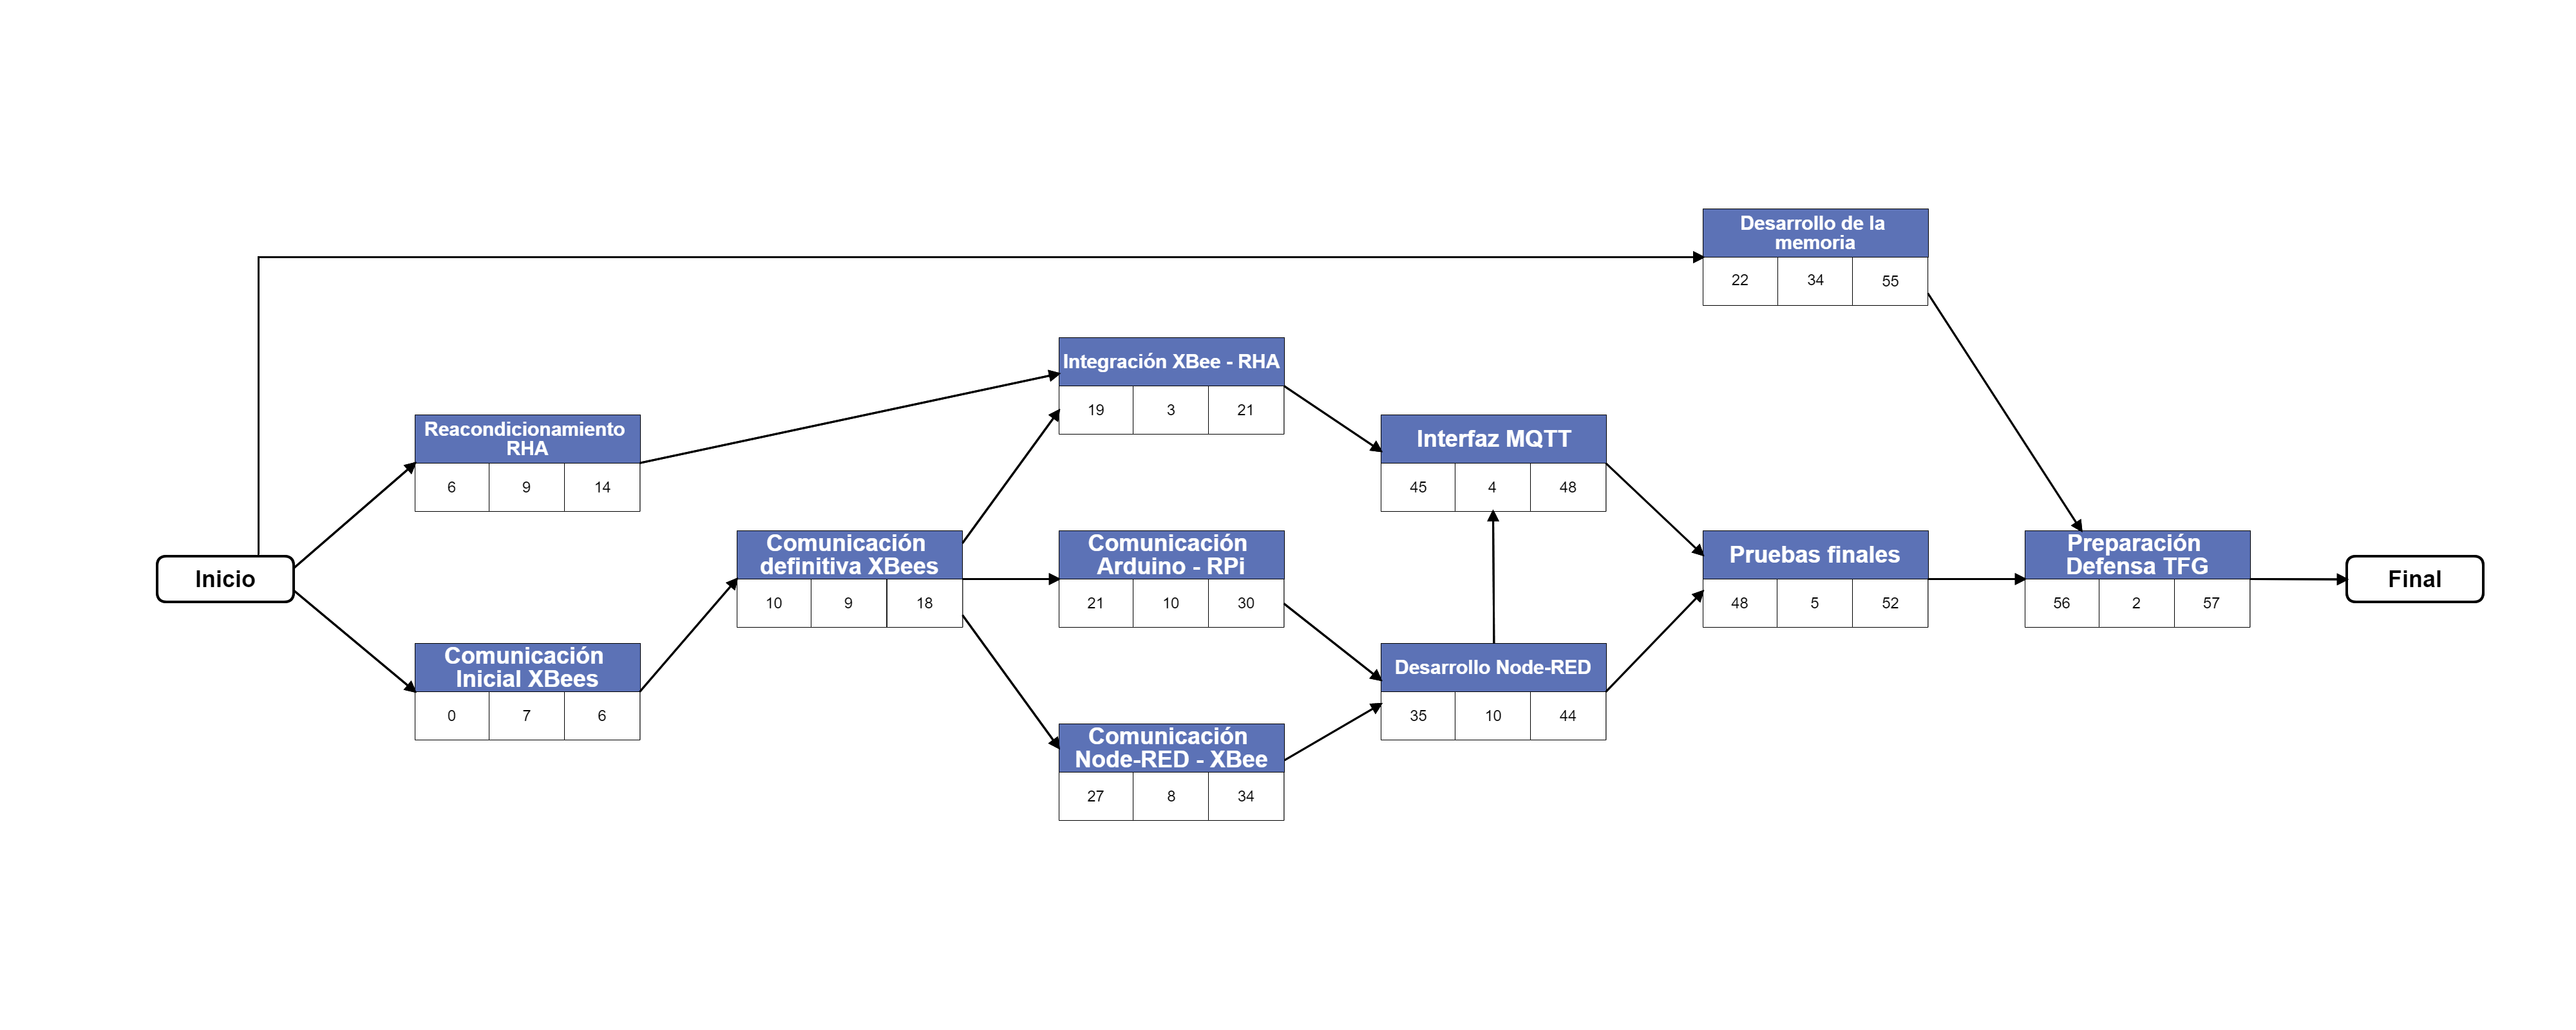
\includegraphics[width=1.7\textwidth]{figuras/Pert.png}
   		\caption{Diagrama de Pert}
   		\label{fig:pert}
   	\end{figure}
\end{landscape}

\section{Planificación}

En el apartado anterior se ha descrito un ciclo de vida del proyecto basado en bloques de tareas. En la figura \ref{fig:gantt} se puede visualizar un Diagrama de Gantt que viene a desglosar estos bloques de tareas y a indicar muy detalladamente su desarrollo temporal.

La disposición anidada de las subtareas que conforman tareas (y que, a su vez, conforman bloques de tareas) encaja con una planificación desde la perspectiva del llamado \textbf{método en V}. Mencionado método es muy usado en el campo de la Ingeniería del Software y por empresas líderes en sus respectivos sectores.

El objetivo es obtener un producto validado y fiable revisando sus requisitos en varios niveles de abstracción. Con recursos temporales y económicos limitados, la minimización de riesgos del proyecto se convierte en vital y el proceso hasta llegar a la implementación tiene que ser llevado con mucha atención. En la rama izquierda de la figura \ref{fig:v} se definen las necesidades a cubrir y las especificaciones del sistema, desde un nivel muy general hasta el diseño en detalle de cada subsistema. A continuación se lleva a cabo la implementación. Posteriormente, se procede a la validación mediante test.

El método en V está diseñado para que si alguna parte no supera los test de validación, se devuelva a su etapa de diseño y sea adaptada hasta superar los mismos.

\begin{figure}[H]
	\centering
   	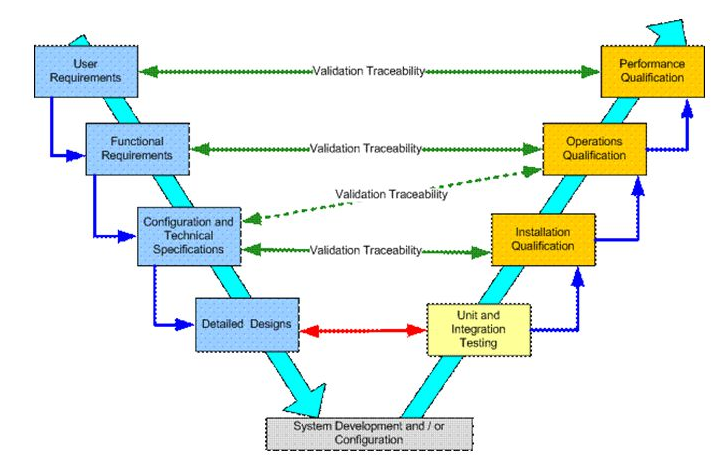
\includegraphics[width=0.8\textwidth]{figuras/v.png}
   	\caption{Método en V}
   	\label{fig:v}
\end{figure}

\begin{landscape}
   	\begin{figure}[H]
   		\centering
   		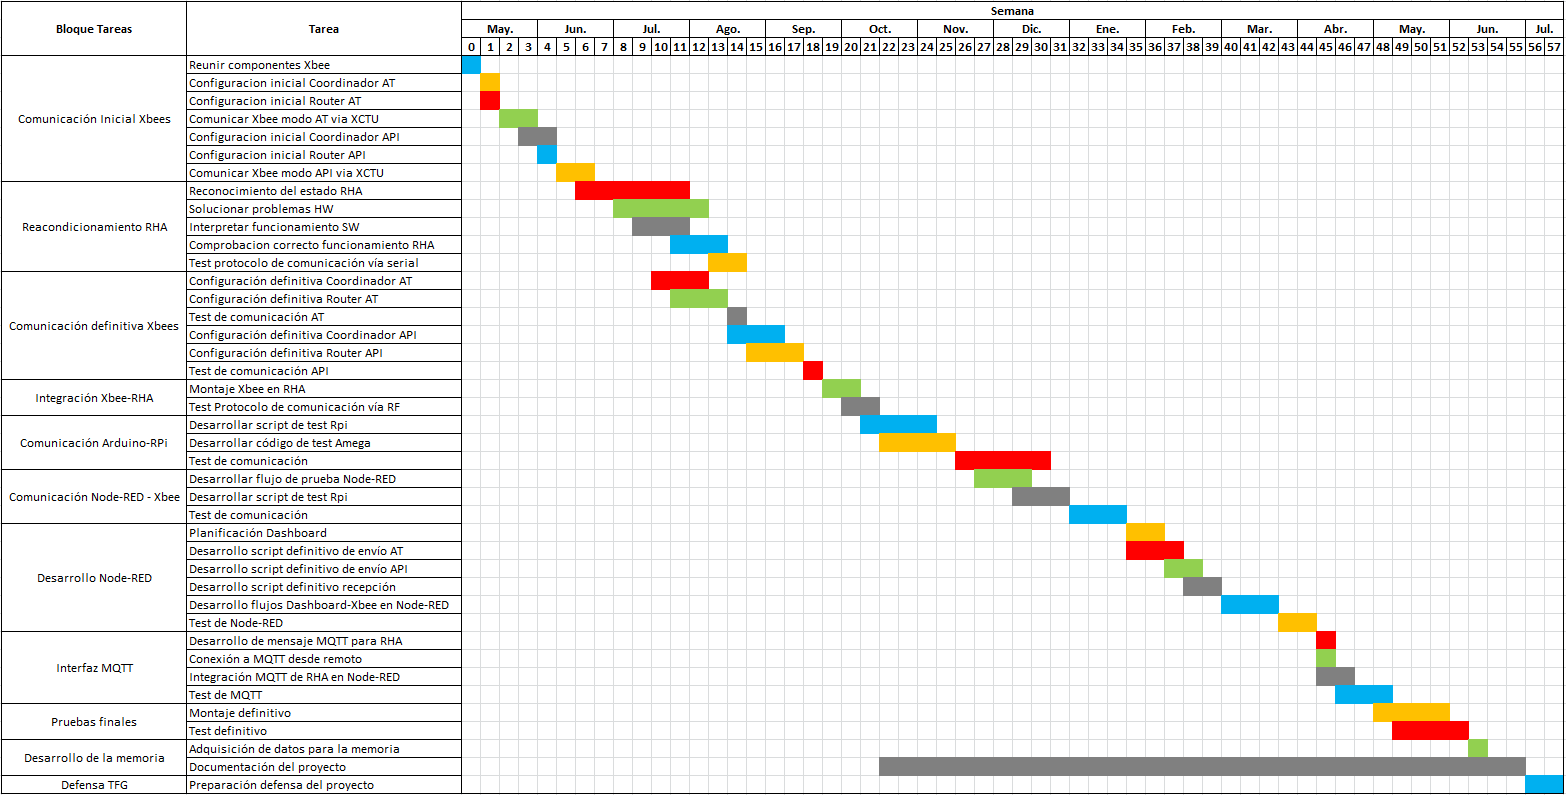
\includegraphics[width=1.6\textwidth]{figuras/Gantt.png}
   		\caption{Diagrama de Gantt}
   		\label{fig:gantt}
   	\end{figure}
\end{landscape}

\section{Presupuesto}

El presupuesto de los componentes del proyecto no es excesivamente largo al estar formado en gran parte por software.

Se tiene en cuenta, no sólo el material que necesita el proyecto para funcionar, sino también el material requerido para su configuración y puesta en marcha. En el caso de realizar más de un prototipo, esto no sería necesario.

Se ha tendido a buscar alternativas en webs oficiales, pese a que fuera posible encontrar los materiales por menor precio. El coste final representa, por lo tanto, un presupuesto máximo para el proyecto.

En la tabla \ref{tab:presupuesto} queda reflejado todo esto de manera ordenada.

\begin{table}[H]
\begin{center}
\begin{minipage}{\textwidth}
\begin{tabular}{|c|c|c|c|c|}
\hline
\textbf{Artículo} & \textbf{Referencia} & \textbf{Coste Unitario}\footnote{En los casos en qué ha sido necesario, se ha aplicado el cambio a Euros oficial propuesto por \cite{bancoEspana} a 24 de junio 2019.} & \textbf{Cantidad} & \textbf{Total} \\
\hline
\hline
Arduino UNO Rev3 & A000066 & 24.20 \euro\footnote{Precios consultados en \cite{arduinoStore} a 24 de junio 2019.} & 2 & 48.40 \euro\\
\hline
Arduino XBee Shield & \multirow{2}{*}{A000007} & \multirow{2}{*}{36.18 \euro\footnote{Precios consultados en \cite{arduinoStore} a 24 de junio 2019.}} & \multirow{2}{*}{2} & \multirow{2}{*}{72.36 \euro}\\
\cline{1-1}
XBee ZB S2C TH\footnote{No se trata exactamente del módulo usado en el proyecto, sino del equivalente actualmente en stock} & & & & \\
\hline
Jumpers de conexión &  - & -  & - & - \\
\hline
& & & Total: & 120.76 \euro\footnote{IVA incluido} \\
\hline
\end{tabular}
\end{minipage}
\end{center}
\caption{Costes del proyecto}
\label{tab:presupuesto}
\end{table}



